\documentclass[11pt, oneside]{article}   	% use "amsart" instead of "article" for AMSLaTeX format
\usepackage[margin=.90in]{geometry}                		% See geometry.pdf to learn the layout options. There are lots.
\geometry{letterpaper}                   		% ... or a4paper or a5paper or ... 
\usepackage[parfill]{parskip}    		% Activate to begin paragraphs with an empty line rather than an indent
\usepackage{graphicx}				% Use pdf, png, jpg, or eps� with pdflatex; use eps in DVI mode
								% TeX will automatically convert eps --> pdf in pdflatex		
\usepackage{amssymb}
\usepackage{graphicx}
\usepackage{xcolor,cancel}
\usepackage{amsmath}
\usepackage{slashed}
\usepackage{listings}
\lstset{language=R}
%\usepackage[section]{placeins}

\newcommand\hcancel[2][black]{\setbox0=\hbox{$#2$}%
\rlap{\raisebox{.45\ht0}{\textcolor{#1}{\rule{\wd0}{1pt}}}}#2}

\usepackage{listings}             % Include the listings-package
\lstset{language=matlab}          % Set your language ( you can change the language for each code-block optionally )
\lstset{showspaces=false, showtabs=false, breaklines=true}

\title{Stat 243: Building an adaptive rejection sampler}
\author{James Bladen, Lisa Felberg, Siwei Tu, Hsin-Wei Tsao}
\date{December 13, 2013}							% Activate to display a given date or no date

\begin{document}
\maketitle

%%%%%%%%%%%%%%%

\section{Introduction}

\subsection*{ (i) }

Adaptive Rejection sampling was first introduced in 1992 by Gilks and Wild.  It was proposed as an alternative to vanilla rejection sampling for functions that are difficult to evaluate multiple times.  The objective of this method is to sample from a "difficult" distribution by representing it with tangent lines and evaluating the actual function as few times as possible.  The basic algorithm is as follows:

\begin{center}
	\begin{itemize}
		\item{ Take the log of the function to sample from, $h(x) = log(f(x))$ }
		\item{ Select two starting points, $x_1$ and $x_2$ that are to the right and to the left of the function's maximum, respectively}
		\item{ Sample two random numbers, one from the uniform random number distribution, URN, and one from the  normalized exponential of the upper bounded line, $x^*$ }
		\item{ If $URN \le exp(l(x*)-u(x*))$, accept and add $x^*$ to vector of $x$'s }
		\item{ Else if $URN \le exp(h(x*)-u(x*))$, accept and add $x^*$ to vector of $x$'s }
		\item{ Else reject }
		\item{ Continue to sample numbers and testing procedure until a desired number of samples is obtained}
	\end{itemize}
\end{center}

The image below is a graphical representation of the algorithm.

\begin{figure}[htbp!]
  \centering
  \caption{ Algorithm of ARS method}
    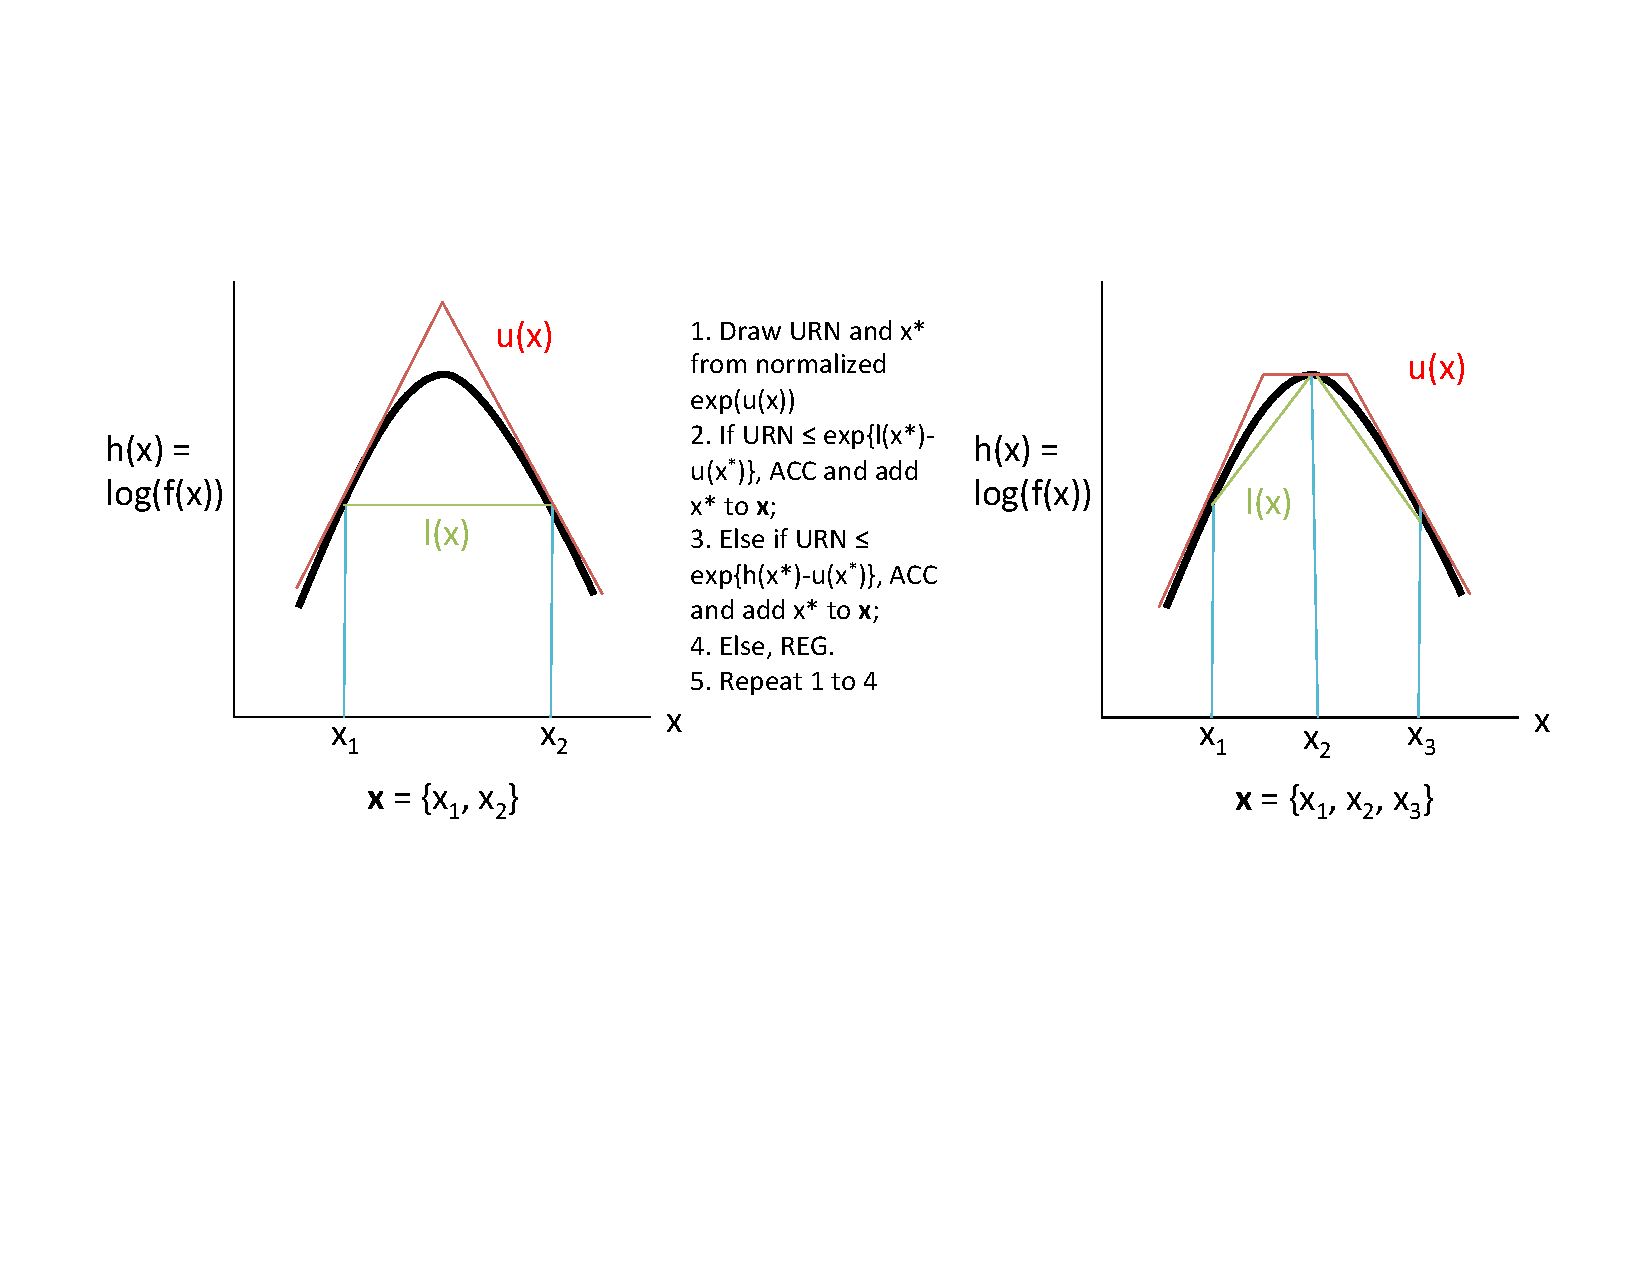
\includegraphics[width=.93\textwidth]{algorithm}
\end{figure}


%%%%%%%%%%%%%%%

\section{Code Structure}

We decided to utilize the S4 class as a format for our code.  It was chosen because of the formal structure and modularity.  These properties also made it easy to test and create in a very piecewise manner.  The general structure to the code is a follows:  A wrapper function \textit{a\_r\_s} runs the sampling method.  The program is run as follows:

 $$sample\gets ars( \mathbf{n}, \mathbf{f\_x}, \mathbf{bounds},\mathbf{guess\_of\_mode}) $$
where\\ 
 $\mathbf{n}=\{\# \, of \, samps \, desired \}, \mathbf{f\_x} = \{f(x) \, to \, sample\}, $\\ $\quad \mathbf{bounds}= \{ bds \, of \, f(x)\, \},   \mathbf{guess\_of\_mode}= \{user's\, guess \,of \,function \, mode\}$
 
 This will return a \textit{Cadapt\_reject\_sample} class which contains sampled points in \textit{ars@samples}.  The class itself contains all the methods and variables required to perform adaptive rejection sampling.  
 
 First, two points are chosen as starting $x_1$ and $x_2$ values.  Next, $x^*$ values are drawn from the corresponding $u(x)$ distribution and the sampling criteria is tested.  This is repeated until the desired number of samples is obtained.    Brief descriptions of the most important methods are given below.  We've included more detailed source documentation as part of our solution as well (see \textit{a\_r\_sManual.pdf}).

\subsection*{ gen\_x method }
In this method, we generate starting points according to user's input of bounds and guess of mode. \\
There are 4 possible cases:
  \begin{itemize}
  \item  If the target function is bounded on both sides, then we take 2 bounds as $x_{1}$, $x_{2}$.
 \end{itemize}
If the target function is unbounded on either one or both sides, we make use of user's guess of mode to find the maximum of target function $f(x)$ (In theory, it should be the real mode.) by applying $optimize(\,)$ and use $(mode-100, mode+100)$ as bounds in the optimize function. The idea is to find the appropriate starting points more quickly.


 \begin{itemize}

  \item  If the target function is unbounded on both sides,  we set $x_{1}$ close to $maxf(x)$. If $h'(x_{1})>0$ then find an $x_{2}$ on the right side of $x_{1}$ s.t. $h'(x_{2})<0$. Similary, if $h'(x_{1})<0$ then find an $x_{2}$ on the left side of $x_{1}$ s.t. $h'(x_{2})>0$. In addition, if $h'(x_{1})=0$ which means $h(x)$ is symmetric to $x_{1}$, then we set $(x_{1}-\frac{1}{2},x_{1}+\frac{1}{2})$ to be 2 starting points.


  \item  If the target function is bounded only on left side,  and if the bound is less than $maxf(x)$, then we use the $maxf(x)$ as $x_{1}$, and find an $x_{2}$ on the right side of $maxf(x)$ s.t. $h'(x_{1})h'(x_{2})<0$. Or, if the bound is greater than $maxf(x)$, we just use the bound as as $x_{1}$, and find an $x_{2}$ on the right side of $maxf(x)$ s.t. $h'(x_{1})h'(x_{2})<0$.

  \item  If the target function is bounded only on right side,  and if the bound is greater than $maxf(x)$, then we use the $maxf(x)$ as $x_{1}$, and find an $x_{2}$ on the right side of $maxf(x)$ s.t. $h'(x_{1})h'(x_{2})<0$. Or, if the bound is smaller than $maxf(x)$, we just use the bound as as $x_{1}$, and find an $x_{2}$ on the right side of $maxf(x)$ s.t. $h'(x_{1})h'(x_{2})<0$.

 \end{itemize}

Note that $h(x)=log(f(x))$ which is concave. So for any $x_1, x_2$, if $h'(x_1)h'(x_2)<0$, $x_1$ and $x_2$ would be on the different side of maximum of $h(x)$. And with the options of 2 to 4, we save $x$, $h(x)$ and $h'(x)$ for all $x$'s we computed in the process for updating our upper and lowr function.


\subsection*{ ev\_h method }
In this method, we calculate the values of $h(x)$ and $h'(x)$ for any $x$ with $genD(\,)$ in package $numDeriv$.

\subsection*{ s\_x method }
In this method, we calculate $s_{k}(x)$ by normalizing $e^{ u_{k}(x)}$. To normalize the $e^{ u_{k}(x)}$, we integrate each piece of $u(x)$ with following algorithm: \\
First note that $u(x)$ is a piecewise defined function. It is linear in each piece of interval. Actually for $x \in [z_{j-1}, z_j]$, $u(x) = ax+b $, where $a=h'(x_j)$ and $b=h(x_j)- x_j h'(x_j)$. \\
So for $x \in [z_{j-1}, z_j]$, 
\begin{displaymath}
\int_{z_{j-1}}^{z_j} \, e^{u(x)} dx =\left. \frac{1}{h'(x_j)} \, exp( h'(x_j)x + h(x_j) -x_j h'(x_j))  \right|_{z_{j-1}}^{z_j},
\end{displaymath}
and
\begin{displaymath}
\int_D e^{u_k(x')} dx' = \left.\sum_j \frac{1}{h'(x_j)} \,exp( h'(x_j)x + h(x_j) -x_j h'(x_j))  \right|_{z_{j-1}}^{z_j}.
\end{displaymath}

In the special case of $a=0$ which means that for $x \in [z_{j-1}, z_j]$, $u(x) = b $ where $b=h(x_j)$. \\Then
\begin{displaymath}
 \int_{z_{j-1}}^{z_j} \, e^{u(x)} dx =\left. e^bx_j\right|_{z_{j-1}}^{z_j} , 
\end{displaymath}
and, 
\begin{displaymath}
\int_D e^{u_k(x')} dx' =\left.\sum_j  e^bx_j\right|_{z_{j-1}}^{z_j}.
\end{displaymath}


\begin{figure}[htbp!]
\clearpage
  \centering
  \caption{ Testing of inverse CDF algorithm I}
    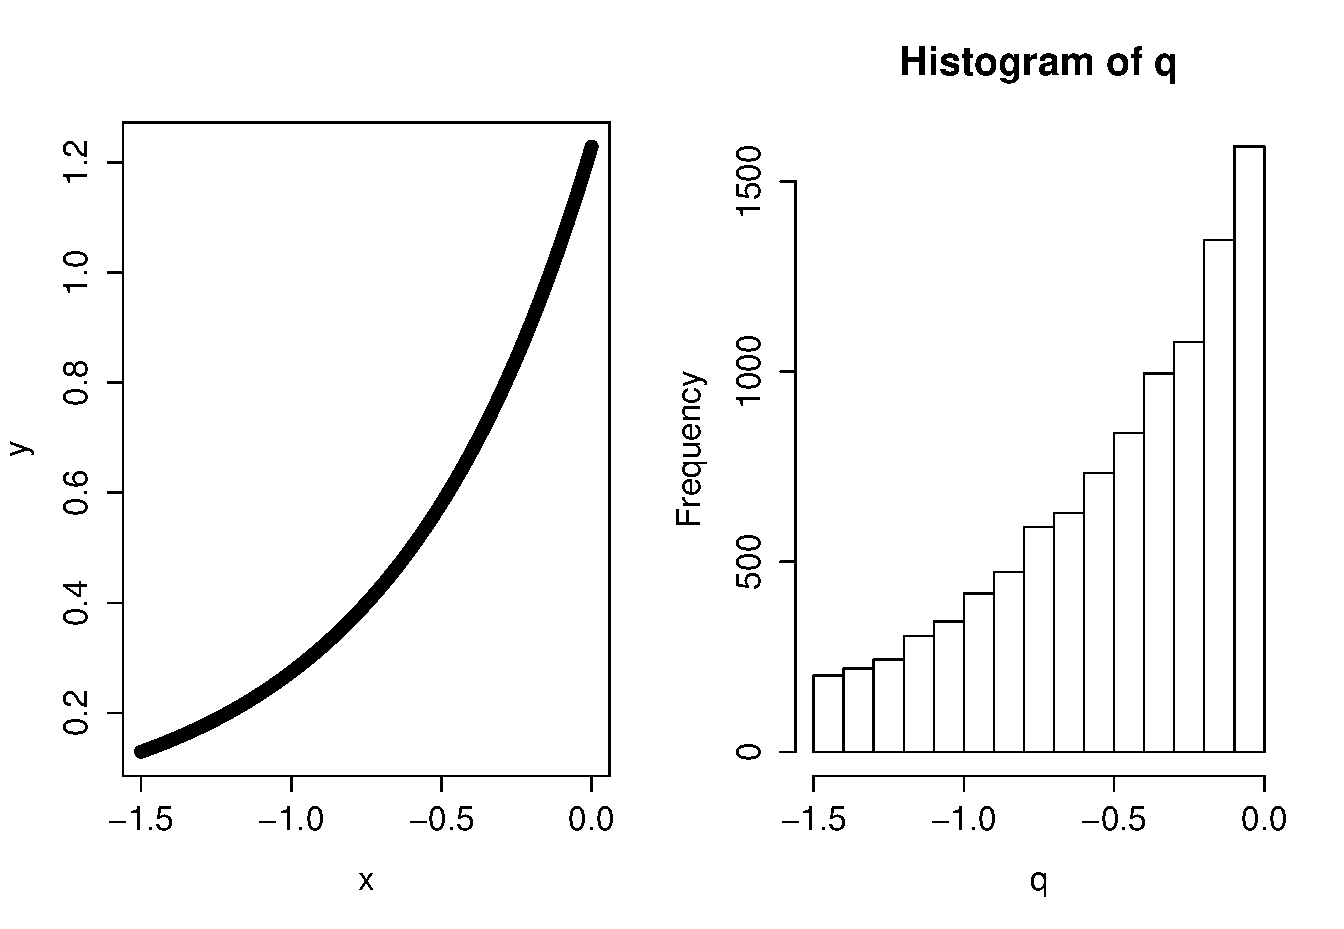
\includegraphics[width=.73\textwidth]{inverse_CDF_1}
\end{figure}

\begin{figure}[htbp!]
\clearpage
 \centering
 \caption{ Testing of inverse CDF algorithm II}
   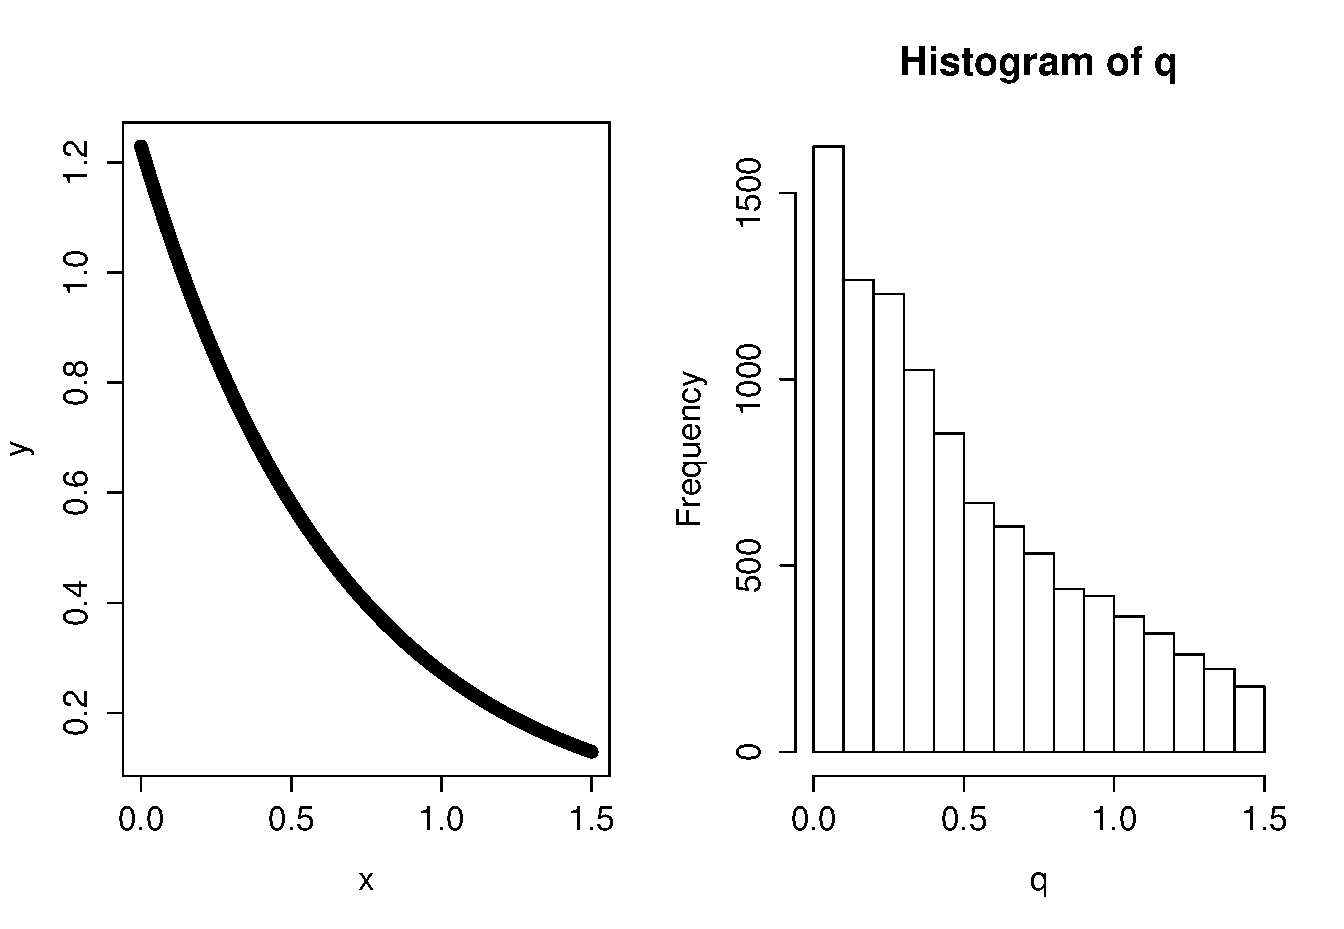
\includegraphics[width=.73\textwidth]{inverse_CDF_2}
\end{figure}



\subsection*{ sampling method }
In this method, we sample a new $x^{*}$ from the $s_{k}(x)$ by using inverse CDF of  $s_{k}(x)$ with a random value $u \sim unif(0,1)$. Moreover, the inverse CDF algorithm we use is as follow: \\
Once we decided which interval $x^*$ falls in, we want to sample from $\frac{e^{u(x)}} {\int e^{u(x)} dx}$. Suppose $x^* \in [z_{j-1}, z_j]$, then $u(x) = ax+b $, where $a=h'(x_j)(\neq0)$ and $b=h(x_j)- x_j h'(x_j)$. \\
Let
\begin{displaymath}
C=\int_{z_{j-1}}^{z_j} \, e^{u(x)} dx,
\end{displaymath}
then the pdf is
\begin{displaymath}
\frac{e^{ax+b}}{C}.
\end{displaymath}
So the CDF
\begin{displaymath}
F'(x)=\int_{z_{j-1}}^{x'} \,  \frac{e^{ax+b}}{C} \, dx = \left. \frac{1}{ca}\, e^{ax+b} \, \right|_{z_{j-1}}^{x'} = \frac{ca}{e^b}\,(e^{ax'}-e^{az_{j-1}}).
\end{displaymath}
Then the inverse of $F(x')$ will be
\begin{displaymath}
\frac{\log\,(\frac{ac}{e^b}+e^{az_{j-1}})}{a}.
\end{displaymath}


In the special case of $a=0$ which means that for $x^* \in [z_{j-1}, z_j]$, $u(x) = b $ where $b=h(x_j)$. \\Then the pdf will be  be $ \frac{e^b}{c}x $ which is an uniform distribution in $[z_{j-1}, z_j]$. In this situation, we just sample $x^*$ from $unif \sim  (z_{j-1}, z_j)$.





\subsection*{ upper method }
In this method, we calculate the $u_{k}(x)$ for $x^*$ which we sample from the sampling method.


\subsection*{ lower method }
In this method, we calculate the $l_{k}(x)$ for $x^*$ which we sample from the sampling method.


\subsection*{ update method }
In this method, we test the sample element $x^{*}$ from sampling method. If it is accepted in the first ratio,  we add the $x^{*}$ into the set of outputs. If it is rejected, then we calculate $h(x)$ and $h'(x)$, we then test for log concavity by seeing if $h(x)$ is between $u(x)$ and $l(x)$, then we create a new ratio and test our $x^*$, if it accepted we add it to the output and update our upper and lower bounds. If it is rejected, we update our bounds but do not put it in the output.



%%%%%%%%%%%%%%%

\section{Testing}

For testing, we rigorously tested each method to ensure it was functioning properly.  To test the overall function, we sampled over a few well known distributions with different bounds, including:  normal, gamma, truncated normal.  The results are shown below.\\
First we test the standard normal with varying bounds , the code to do so and the histogram of the resulting samples are given below: \newline

\begin{lstlisting}[frame=single]
samples <- ars(n=10000,fx=function(x){(1/sqrt(2*pi)*exp((-(x-0)^2)/2))}, bounds=c(-Inf, Inf) )
sample<-ars(10000,function(x){(1/sqrt(2*pi)*exp((-(x-0)^2)/2))},c(-2, 2))
sample<-ars(10000,function(x){(1/sqrt(2*pi)*exp((-(x-0)^2)/2))},c(-Inf, 2))
sample<-ars(10000,function(x){(1/sqrt(2*pi)*exp((-(x-0)^2)/2))},c(-2, Inf))


\end{lstlisting}
\clearpage
\begin{figure}[htbp!]
 \centering
\caption{Histogram of samples from $f(x)=\frac{1}{\sqrt{2\pi}}e^{-\frac{x^2}{2}}$ with different bounds}
  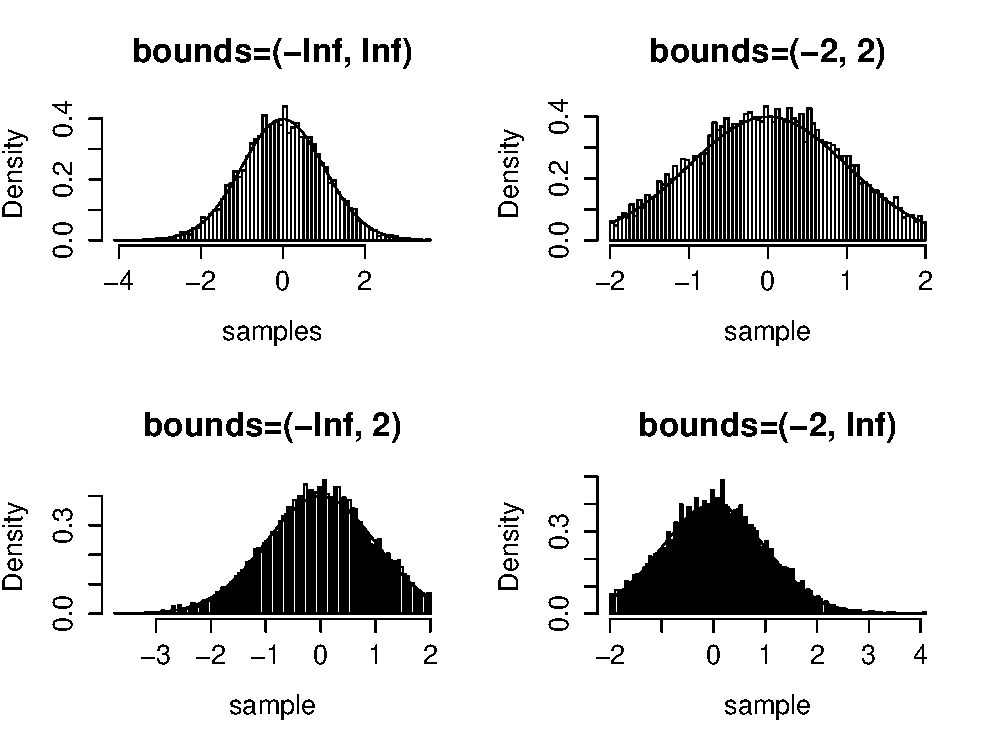
\includegraphics[width=1.0\textwidth]{standardnormal}
\end{figure}


Second we test the gamma(10,10) with a right bound 0.01 and the gamma(4,5) with bounds (0.8,3), the code to do so and the histogram of the resulting samples are given below:\newline

\begin{lstlisting}[frame=single]
sample<-ars(10000,function(x){(10^10)/gamma(10)*x^9*exp(-10*x)},c(0.01, Inf),10)
sample<-ars(10000,function(x){(5^4)/gamma(4)*x^3*exp(-5*x)},c(0.8,3),4)


\end{lstlisting}
\clearpage
\begin{figure}[htbp!]
 \centering
\caption{left: gamma(10,10), right: gamma(4,5)}
  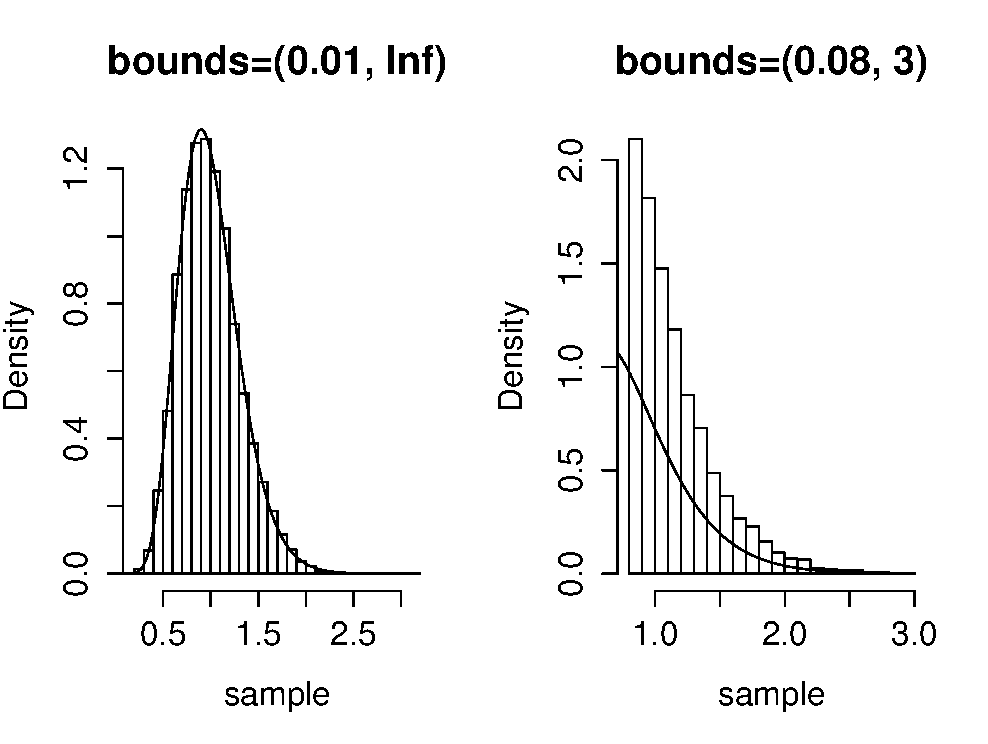
\includegraphics[width=1.0\textwidth]{gamma}
\end{figure}




Third we test the beta(10,10) with bounds$=(0,1)$ and the chi-square (df=10) with a right bound 0, the code to do so and the histogram of the resulting samples are given below: \newline

\begin{lstlisting}[frame=single]
sample<-ars(10000,function(x){x^9*(1-x)^9/beta(10,10)},c(0,1))
sample<-ars(10000,function(x){1/(2^5*gamma(5))*x^4*exp(-x/2)},c(0,Inf))




\end{lstlisting}
\clearpage
\begin{figure}[htbp!]
 \centering
\caption{left: beta(10,10), right: chi-square(df=10)}
  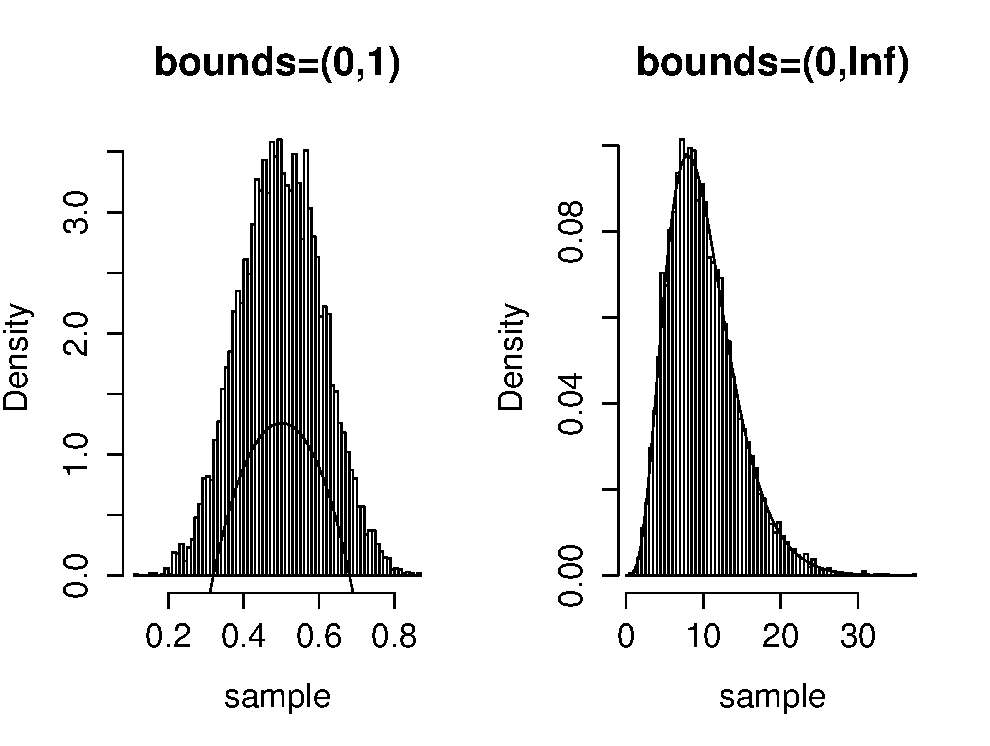
\includegraphics[width=1.0\textwidth]{betachi}
\end{figure}

For the gamma(4,5) and beta distribution, you may note that the plotted distribution curve falls below the sampled histogram, this is simply because the density is not normalized.  But it is immediately apparent that the samples follow the same trend as the curve.  

For methods testing, we have included in our final solution some simple lines of code to run, testing methods individually.  Please see our source code for more details.  

%%%%%%%%%%%%%%%

\section{Contributions}

Everyone in the group contributed relatively equally to each aspect of the project.  Some efforts were more focused as follows:

\subsection*{Code writing}

General structure: Lisa

Methods: James, Siwei, Hsin-Wei

\subsection*{Code testing}

Methods testing: James, Siwei

Overall function tests: Lisa, Hsin-Wei

\subsection*{Documentation} 

Manual creation: Lisa

Project write-up:  Hsin-Wei, Lisa

\end{document}


%\begin{lstlisting}
%x = 0:0.1:100;
%m = 0:19;
%
%y = zeros(1,1001);
%
%for i = 1:1001
%    xis = (0.05.*( 1 + x( i )  ) ).^m ;
%    y(i) = (((0.05.*( 1 + x( i )  ) ).^20 ) * ((1/x(i) + 10^4)/( 1/x(i) + 1 )))  /(sum( xis  ) + (((0.05.*( 1 + x( i )  ) ).^20 ) * ((1/x(i) + 10^4)/( 1/x(i) + 1 ))) );
%end
%
%plot( x, y)
%
%\end{lstlisting}

%\begin{figure}[htbp!]
%  \centering
%  \caption{ Plot of P(M*) versus x for strong binding}
%    \includegraphics[width=.73\textwidth]{chem220_ps7_4_2}
%\end{figure}


